\begin{thm}{159}{\hosi 7}{JMO予選 2017-8}
 $\triangle\mr{ABC}$の辺$\mr{BC}$上に4点$\mr{B}, \mr{D}, \mr{E}, \mr{C}$がこの順にならぶ。$\triangle\mr{ABE}$の外接円と$\triangle\mr{ADC}$の外接円の、$\mr{A}$と異なる交点を$\mr{X}$、$\mr{AX}$と$\mr{BC}$の交点を$\mr{F}$とする。$\angle\mr{BAD}=\angle\mr{ACE}$, $\angle\mr{ABD}=\angle\mr{CAE}$, $\mr{BF}=5$, $\mr{CF}=6$, $\mr{XD}=3$ のとき、$\mr{XE}$を求めよ。
\end{thm}

$\angle\mr{ACE}=\angle\mr{BAD}=\theta$, $\angle\mr{CAE}=\angle\mr{ABD}=\phi$とおく。また$\triangle\mr{ABE}$の外接円を$C_1$、$\triangle\mr{ADC}$の外接円を$C_2$とおく。
\begin{figure}[H]
 \centering
 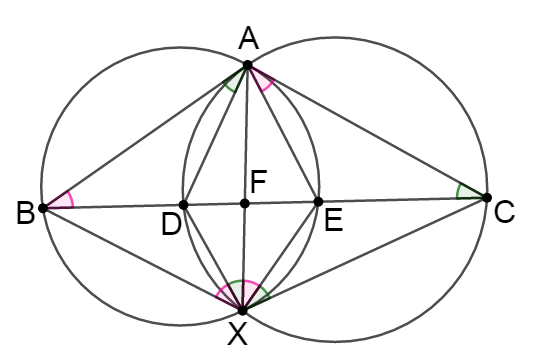
\includegraphics[width=0.8\linewidth]{../problems/Q_159/A_159.png}
\end{figure}
$\angle\mr{ADE}=\angle\mr{AED}=\theta+\phi$となっているから、$\mr{AD}=\mr{AE}$が成り立つ。円$C_1$で方べきの定理によって$\mr{DF}\cdot\mr{FC}=\mr{AF}\cdot\mr{FX}$。また円$C_2$で方べきの定理によって$\mr{AF}\cdot\mr{FX}=\mr{BF}\cdot\mr{FE}$。これらによって
\[ \mr{DF}\cdot\mr{FC}=\mr{BF}\cdot\mr{FE} \,\dou\, 6\mr{DF}=5\mr{FE} \,\dou\, \mr{DF}:\mr{FE}=5:6 \]

続いて円周角の定理を用いて、$C_2$にて$\angle\mr{AXD}=\angle\mr{ACD}=\theta$、$C_1$にて$\angle\mr{AXE}=\angle\mr{ABE}=\phi$なので、
\[ \angle\mr{DXE}=\angle\mr{AXD}+\angle\mr{AXE}=\theta+\phi \]
$C_1$の別の円周角で$\angle\mr{AXB}=\mr{AEB}=\theta+\phi$であるから、
\[ \angle\mr{DXB}=\angle\mr{AXB}-\angle\mr{AXD}=(\theta+\phi)-\theta=\phi=\angle\mr{AXE} \]
となる。$C_2$でまた別の円周角をみれば、$\angle\mr{XAE}=\angle\mr{XBD}$である。これらより、2つの角が等しいから$\triangle\mr{XAE}\sim\triangle\mr{XBD}$がわかる。

さて、$\mr{DF}=5k$, $\mr{FE}=6k$とおく。明らかに$\mr{BF}>\mr{DF}$だから$0<k<1$。このとき$\mr{BD}=5(1-k)$, $\mr{CE}=6(1-k)$となる。$\triangle\mr{ABD}\sim\triangle\mr{ECA}$であって、$\mr{AD}=\mr{AE}=x$とおいて相似比は、
\[ \mr{BD}:\mr{DA}=\mr{AE}:\mr{EC} \,\dou\, 5(1-k):x=x:6(1-k) \]
よって$x=\sqrt{30}(1-k)$となる。続いて$\triangle\mr{XAE}$と$\triangle\mr{XBD}$の相似比をみて、
\[ \mr{BD}:\mr{DX}=\mr{AE}:\mr{EX} \,\dou\, 5(1-k):3=\sqrt{30}(1-k):\mr{EX} \]
であるから、$\mr{EX}=\dfrac{3}{5}\sqrt{30}$
